\chapter{アップサンプリング}
    \section{アップサンプリングされた信号の周波数特性}
        \newcommand{\xda}{x_{\text{d},1}}
        \newcommand{\Xda}{X_{\text{d},1}}
        \newcommand{\xdb}{x_{\text{d},2}}
        \newcommand{\Xdb}{X_{\text{d},2}}
        \subsection{動機}
            離散時間信号をアップサンプリングしてDACで出力したときの周波数スペクトルを計算したい。
            DACの量子化誤差は無視する。
        \subsection{アップサンプリングされた離散時間信号のDTFT}
            DAC の出力を考える前に、まずは離散時間の領域での様子を調べる。
            結果は驚くほど単純なものになる。
            \par
            記号を次のように定義する。
            \begin{itemize}
                \item $R\in\naturalNumbers,\;R\geq 2$ : アップサンプリングレート
                \item $\xda:\integers\to\complexNumbers$ : 離散時間信号
                \item $\Ts>0$ : $\xda$ のサンプル周期
                \item $\Xda$ : $\xda$ のDTFT
                \item $\xdb$ : $\xda$ を $R$ 倍にアップサンプリング(元の信号のサンプル同士の間に $R-1$ 個の0を追加)した離散時間信号
                \item $\Xdb$ : $\xdb$ のDTFT
            \end{itemize}
            \subsubsection{主張}
                $\Xdb(\omega) = \Xda(\omega)$ が成り立つ。
            \subsubsection{導出}
                \begin{proof}
                    \quad\par
                    $\xda$ のサンプリング周期が $\Ts/R$ であることに注意する。
                    \begin{align*}
                        \Xdb(\omega) &= \sum_{n=-\infty}^\infty \xdb(n)\exp(-i\omega n\Ts/R) = \sum_{m=-\infty}^\infty \xdb(m R) \exp(-i\omega m R\Ts/R) \\
                        &= \sum_{m=-\infty}^\infty \xda(m) \exp(-i\omega m\Ts) = \Xda(\omega)
                    \end{align*}
                \end{proof}
                一般に、サンプリング周期が $\Ts/R$ である離散時間信号の DTFT は $2\pi R/\Ts$ 周期関数であり、当然 $\xdb$ についてもそれは成り立っている。
                その上でさらに、$\xdb$ については DTFT が $\xda$ のそれと完全に一致して $2\pi/\Ts$ 周期関数にもなっている。
        \subsection{アップサンプリングされた信号をそのままDAC出力した場合}
            \subsubsection{主張}
                記号を次のように定義する。
                \begin{itemize}
                    \item $R\in\naturalNumbers,\;R\geq 2$ : アップサンプリングレート
                    \item $\xda:\integers\to\complexNumbers$ : 離散時間信号
                    \item $\Ts>0$ : $\xda$ のサンプル周期
                    \item $\Xda$ : $\xda$ のDTFT
                    \item $\xdb$ : $\xda$ を $R$ 倍にアップサンプリング(元の信号のサンプル同士の間に $R-1$ 個の0を追加)した離散時間信号
                    \item $x_1$ : $\Ts$ をサンプル周期として $\xda$ の0次ホールドで生成した階段状の連続時間信号
                    \item $x_2$ : $\Ts/R$ をサンプル周期として $\xdb$ の0次ホールドで生成した階段状の連続時間信号
                \end{itemize}
                $u_1:\realNumbers\to\braces{0,1}$ を幅 $\Ts$ のパルスとする。
                \[
                    u_1(t) = \begin{cases}
                        1 & 0\leq t < \Ts \\
                        0 & \text{otherwise}
                    \end{cases}
                \]
                $u_2:\realNumbers\to\braces{0,1}$ を幅 $\Ts/R$ のパルスとする。
                \[
                    u_2(t) = \begin{cases}
                        1 & 0\leq t < \Ts/R \\
                        0 & \text{otherwise}
                    \end{cases}
                \]
                $x_1$ は次式で表される。
                \[ x_1(t) = \sum_{n=-\infty}^\infty \xda(n)u_1(t-n\Ts) \]
                $x_2$ は次式で表される。
                \[ x_2(t) = \sum_{n=-\infty}^\infty \xdb(n)u_2(t-n\Ts/R) = \sum_{m=-\infty}^\infty \xdb(R m)u_2(t-m\Ts) = \sum_{n=-\infty}^\infty \xda(n)u_2(t-n\Ts) \]
                次の図は $\Ts=1,R=4,\xda(n) = \sin\parens{2\pi*n/12}\;(0\leq n\leq 24),\;\xda(n) = 0\;(n<0,24<n)$ の例である。
                \begin{figure}[H]
                    \centering
                    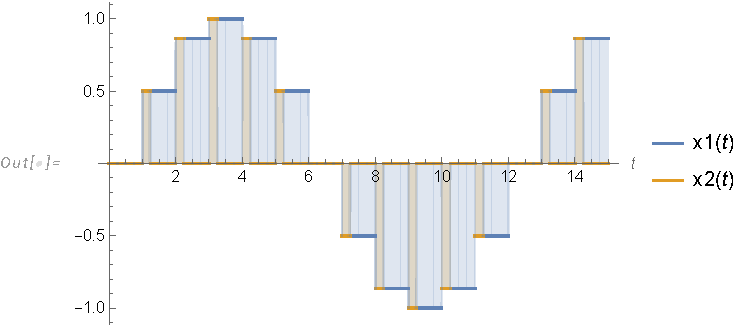
\includegraphics[keepaspectratio, scale=0.8]
                    {\currfiledir/imgs/x1,x2.pdf}
                    \caption{$x_1,x_2$の例}
                    \label{アップサンプリング前後のDAC出力の例}
                \end{figure}
                以上の下、 $x_2$ のFourier変換 $X_2$ は次式である。
                \[ X_2(\omega) = \frac{\Ts}{R\sqrt{2\pi}}\exp\parens*{-i\frac{\Ts}{2R}\omega}\parens*{\sinc \frac{\Ts}{2R}\omega}\Xda(\omega) \]
            \subsubsection{導出}
                \begin{proof}
                    \quad\par
                    \[ X_2(\omega) = \FT{\sum_{n=-\infty}^\infty \xda(n)u_2(t-n\Ts)}(\omega) = \sum_{n=-\infty}^\infty \xda(n)\FT{u_2(t-n\Ts)}(\omega) \]
                    ここで\ref{0次ホールドされた離散時間信号の周波数特性}と同様にして次式が成り立つ。
                    \[ \FT{u_2(t-n\Ts)}(\omega) = \frac{\Ts}{R\sqrt{2\pi}}\exp\parens*{-i \omega n\Ts}\exp\parens*{-i\frac{\omega\Ts}{2R}}\sinc\frac{\omega\Ts}{2R} \]
                    よって次式が成り立つ。
                    \begin{align*}
                        X_2(\omega) &= \sum_{n=-\infty}^\infty \xda(n)\frac{\Ts}{R\sqrt{2\pi}}\exp\parens*{-i \omega n\Ts}\exp\parens*{-i\frac{\omega\Ts}{2R}}\sinc\frac{\omega\Ts}{2R} \\
                        &= \frac{\Ts}{R\sqrt{2\pi}}\exp\parens*{-i\frac{\omega\Ts}{2R}}\parens*{\sinc\frac{\omega\Ts}{2R}} \sum_{n=-\infty}^\infty \xda(n)\exp\parens*{-i \omega n\Ts} \\
                        &= \frac{\Ts}{R\sqrt{2\pi}}\exp\parens*{-i\frac{\omega\Ts}{2R}}\parens*{\sinc\frac{\omega\Ts}{2R}} \Xda(\omega) \tag{a}
                    \end{align*}
                \end{proof}
            \subsubsection{考察}
                アップサンプリング前の信号 $x_1$ については\ref{0次ホールドされた離散時間信号の周波数特性}より、そのFourier変換は次式である。
                \[ X_1(\omega) = \frac{\Ts}{\sqrt{2\pi}}\exp\parens*{-i\frac{\Ts}{2}\omega}\parens*{\sinc \frac{\Ts}{2}\omega}\Xda(\omega) \tag{b} \]
                式(a),(b)を見比べると $\Xda$ を共通して含んでおり、それ以外の箇所でアップサンプリングにより $\Ts$ が $\Ts/R$ に置き換わっていることがわかる。
                このことから、アップサンプリングにより高調波の位置は変わらず、広域の減衰や位相回転が緩やかになることがわかる。
                次の図は\ref{アップサンプリング前後のDAC出力の例}に対応するDTFTとFourier変換の絶対値の例である。
                \begin{figure}[H]
                    \centering
                    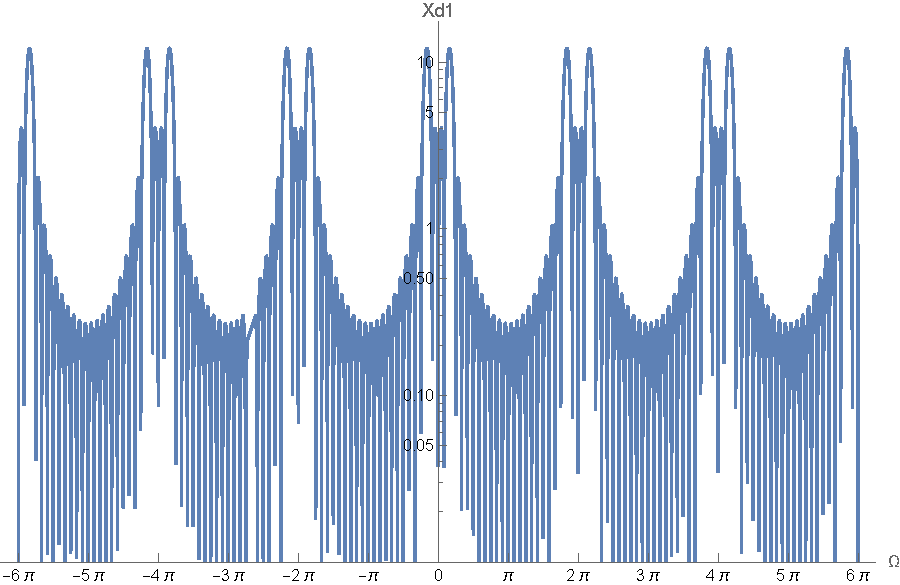
\includegraphics[keepaspectratio, scale=0.8]
                    {\currfiledir/imgs/Xd1.pdf}
                    \caption{$\Xda$の例。横軸は正規化各周波数。}
                \end{figure}
                \begin{figure}[H]
                    \centering
                    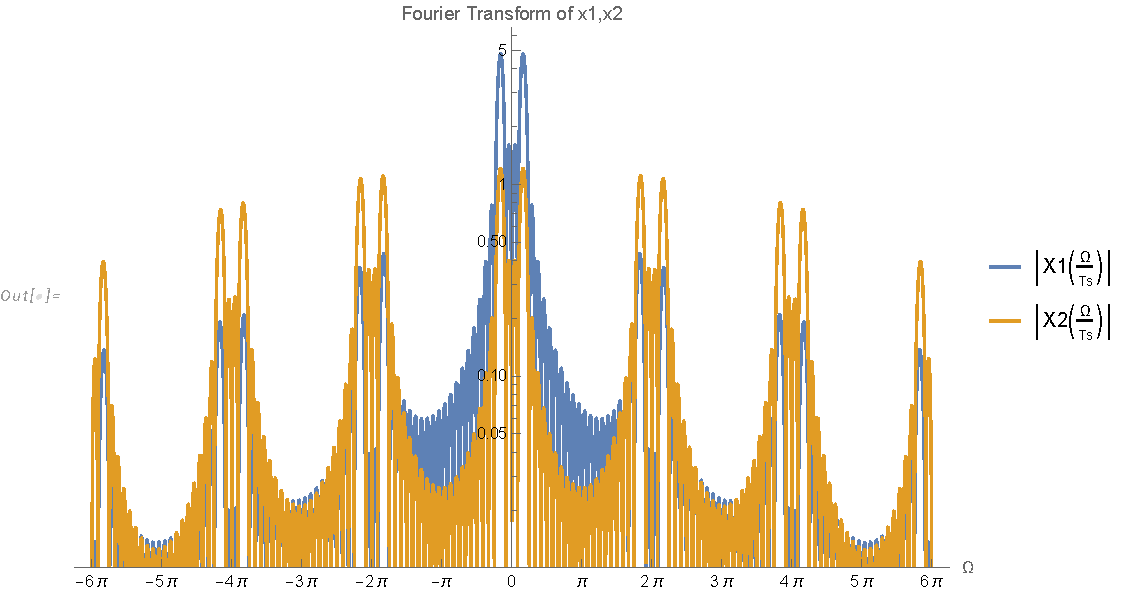
\includegraphics[keepaspectratio, scale=0.8]
                    {\currfiledir/imgs/FT_of_x1,x2.pdf}
                    \caption{$X_1,X_2$の例。横軸は正規化各周波数。}
                \end{figure}